\chapter{map objects}
\label{map} \index{map object}


{\em Authors: Stefan Lang and Andreas Brezger} \\
{\em email: \href{mailto:lang@stat.uni-muenchen.de}{lang@stat.uni-muenchen.de} and \href{mailto:andib@stat.uni-muenchen.de}{andib@stat.uni-muenchen.de}}\\
\vspace{0.3cm}


{\em Map objects} are used to handle and store geographical maps.
For the moment {\em map objects} serve more or less as auxiliary
objects for {\em bayesreg objects} and {\em remlreg objects},
where the effect of spatial covariates on a dependent variable can
be modelled via Markov random field priors. The main purpose of
{\em map objects} in this context is to provide the neighborhood
structure of the map and to compute weights associated with this
neighborhood structure. The typical approach is as follows: A {\em
map object} is created and the boundary information of a
geographical map is read from an external file and stored in the
{\em map object}. This can be achieved using the #infile# command,
see \autoref{mapinfile} below. Based on the boundary information,
the {\em map object} automatically computes the neighborhood structure
of the map and the weights associated with the neighborhood
structure. Since there are several proposals in the spatial
statistics literature for defining the weights, the user is given
the choice between a couple of alternative weight definitions.
After the correct initialization, the {\em map object} can be
passed to the #regress# function of a {\em bayesreg object} in
order to estimate regression models with spatial covariates, see
\autoref{bayesreg}, in particular \autoref{bayesregress}, and the
subsections about spatial covariates therein.

\section{Method infile}
\label{mapinfile} \index{map object!infile command} \index{map
object!boundary files} \index{boundary files} \index{graph files}
\index{reading graph files} \index{reading boundary files}

\subsection{Description}


Method #infile# is used to read the boundary information of a
geographical map stored in an external file. This file is called a
{\em boundary file}, since it must contain the information about
the boundaries of the different regions of the map. It is assumed
that the boundary of each region is stored in form of a closed
polygon, that is the boundary is represented by a set of connected
straight lines. A detailed description of the structure of
boundary files is given below.

As a second choice method #infile# allows to read  so called {\em
graph files}. In {\em graph files} the nodes and edges of a
certain graph are stored. In addition, weights associated with the
edges of the graph may be specified in the file. In terms of
geographical maps the nodes of a graph correspond to the regions
of a map and the edges specify the neighborhood structure of the
map. The main advantage of {\em graph files} is that the
neighborhood structure of a particular geographical map is already
available. With {\em boundary files} the neighborhood structure
must be computed first; a task which is relatively computer
intensive.

Usually {\em boundary files} are read  only once to compute the
neighborhood structure of a geographical map. Having computed the
neighborhood structure, the map can be stored as a {\em graph
file} using the #outfile# command, see \autoref{mapoutfile}. In
subsequent sessions typically the {\em graph file} is used rather
than the corresponding {\em boundary file} because reading {\em
graph files} is less computer intensive.


\subsection{Syntax}

#> #{\em objectname}.#infile# [{\em , options}] #using# {\em filename}

Method #infile# reads the map information stored in the {\em
boundary} or {\em graph file} {\em filename}. If option #graph# is
specified, {\em BayesX} expects a {\em graph file}, otherwise a
{\em boundary file}
is expected. The structures of {\em boundary} and {\em graph files} are described below.

\subsubsection*{Structure of a boundary file}

A {\em boundary file} provides the boundary information of a
geographical map. For each region of the map the {\em boundary
file} must contain the identifying name of the region, the
polygons that form the boundary of the region, and the number of
lines the polygon consists of. The first line always contains the
region code surrounded by quotation marks and the number of lines
the polygon of the region consists of. The code and the number of
lines must be separated by a comma. The subsequent lines contain
the coordinates of the straight lines that form the boundary of
the region. The straight lines are represented by the coordinates
of their end points. Coordinates must be separated by a comma.

To give an example we print a (small) part of the {\em boundary
file} of Germany:


\footnotesize

\hspace{1cm}  $\vdots$

"6634",31 \\
2319.26831,4344.48828 \\
2375.45435,4399.50391 \\
2390.67139,4446.32520 \\
2470.26807,4405.35645 \\
2576.78735,4379.60449 \\
2607.22144,4337.46533 \\
2627.12061,4356.19385 \\
2662.23682,4355.02344 \\
2691.50024,4311.71338 \\
2726.61646,4310.54248 \\
2716.08154,4256.69775 \\
2710.22900,4227.43408 \\
2680.96533,4234.45752 \\
2583.81055,4165.39551 \\
2568.59351,4096.33398 \\
2520.60132,4042.48901 \\
2535.81836,3941.82251 \\
2490.16724,3920.75269 \\
2451.53955,3903.19458 \\
2437.49292,3924.26440 \\
2369.60156,3933.62866 \\
2359.06665,3951.18677 \\
2285.32275,3969.91553 \\
2258.40015,4061.21753 \\
2197.53223,4049.51221 \\
2162.41602,4086.96948 \\
2204.55542,4091.65161 \\
2192.85010,4125.59717 \\
2284.15210,4220.41113 \\
2339.16748,4292.98438 \\
2319.26831,4344.48828

\hspace{1cm} $\vdots$

\normalsize

\vspace{0.3cm}

The  map corresponding to the section of the {\em boundary file}
above can be found in \autoref{partgermany}. Note that the first
and the last point must be identical (see the example above) to
obtain a closed polygon.


\begin{figure}[ht]
\centering
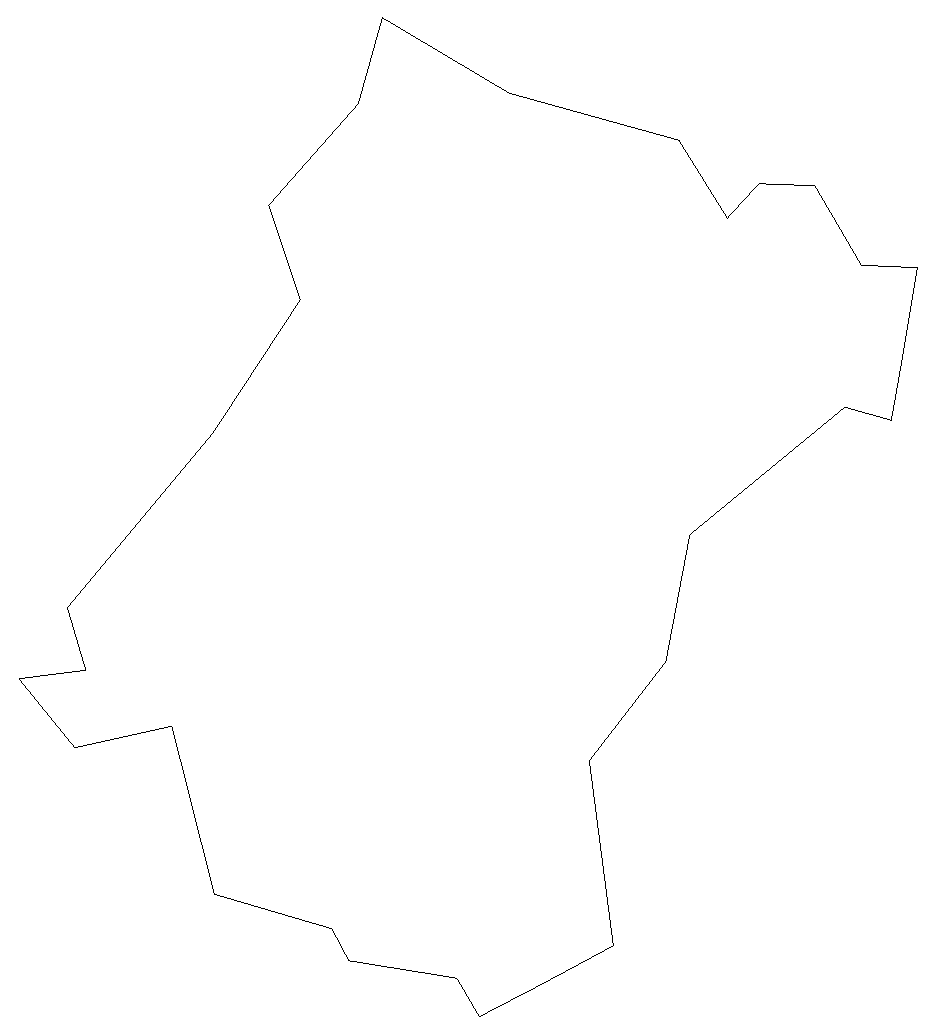
\includegraphics [scale=0.3]{grafiken/westpart.eps}
{\em\caption{\label{partgermany} Corresponding graph of the
section of the boundary file}}
\end{figure}

In some cases it might happen that a region is separated into
subregions that are not connected. As an illustrative example
compare \autoref{westsub} showing a region of Germany that is
separated into 8 subregions. In this case the {\em boundary file}
must contain the polygons of all subregions. The first row for
each of these subregions must contain the region code and the
number of lines the polygon of the respective subregion consists
of. Note that it is not necessary that the polygons of the
subregions are stored in subsequent order in the {\em boundary
file}.

Another special case that might occur is illustrated in
\autoref{westin}. Here a region is completely surrounded by
another region. In this case an additional line must be added to
the boundary description of the {\em surrounded} region. The
additional line must be placed  after the first line and must
contain the
region code of the {\em surrounding} region. The syntax is:

#is.in#,"{\em region code}"

The following lines show a section of the {\em boundary file} of
Germany, where region "9361" is totally
surrounded by region "9371":

\footnotesize

\hspace{1cm} $\vdots$

"9361",7 \\
is.in,"9371" \\
4155.84668,2409.58496 \\
4161.69922,2449.38330 \\
4201.49756,2461.08862 \\
4224.90820,2478.64673 \\
4250.66016,2418.94922 \\
4193.30371,2387.34448 \\
4155.84668,2409.58496

\hspace{1cm} $\vdots$

\normalsize

\begin{figure}[hb]
\centering
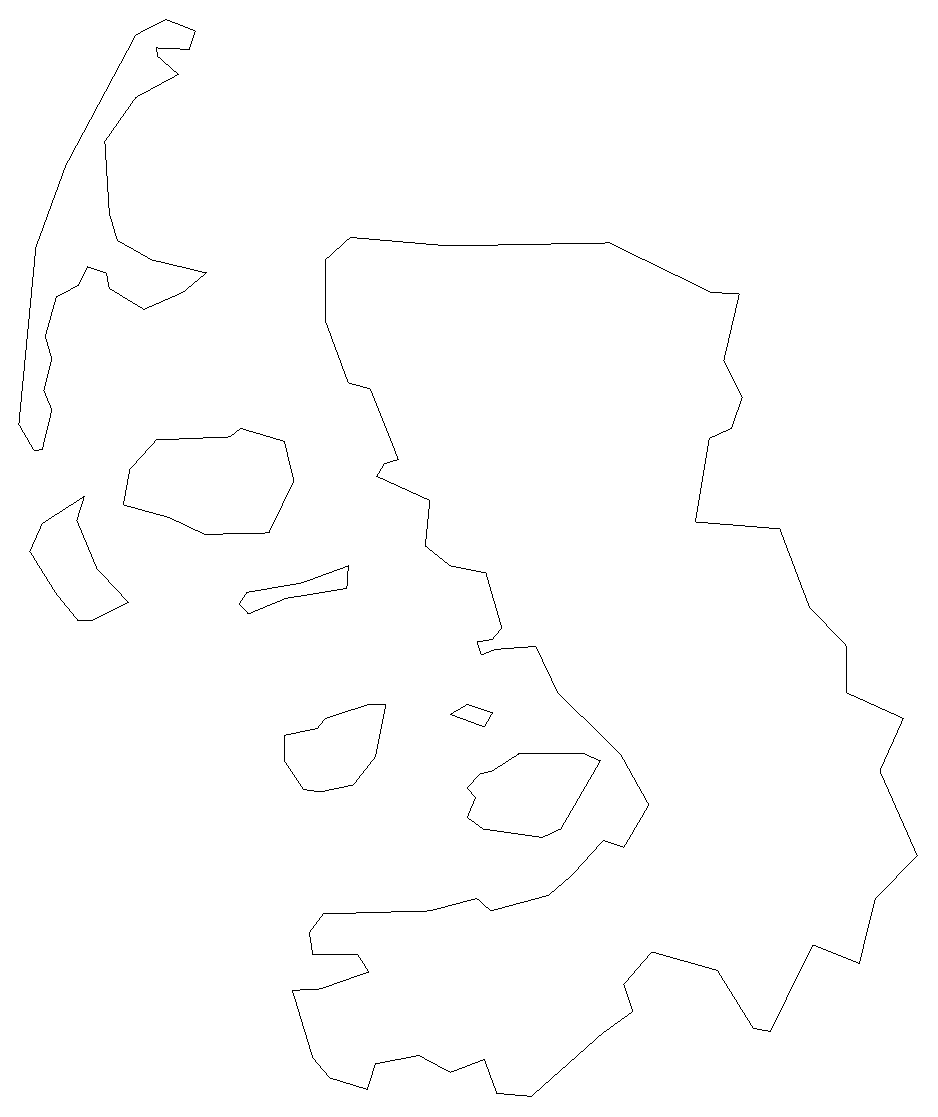
\includegraphics [scale=0.3]{grafiken/reg1054.eps}
{\em\caption{\label{westsub} Example for a region that is divided
into subregions}}
\end{figure}

\begin{figure}[hb]
\centering
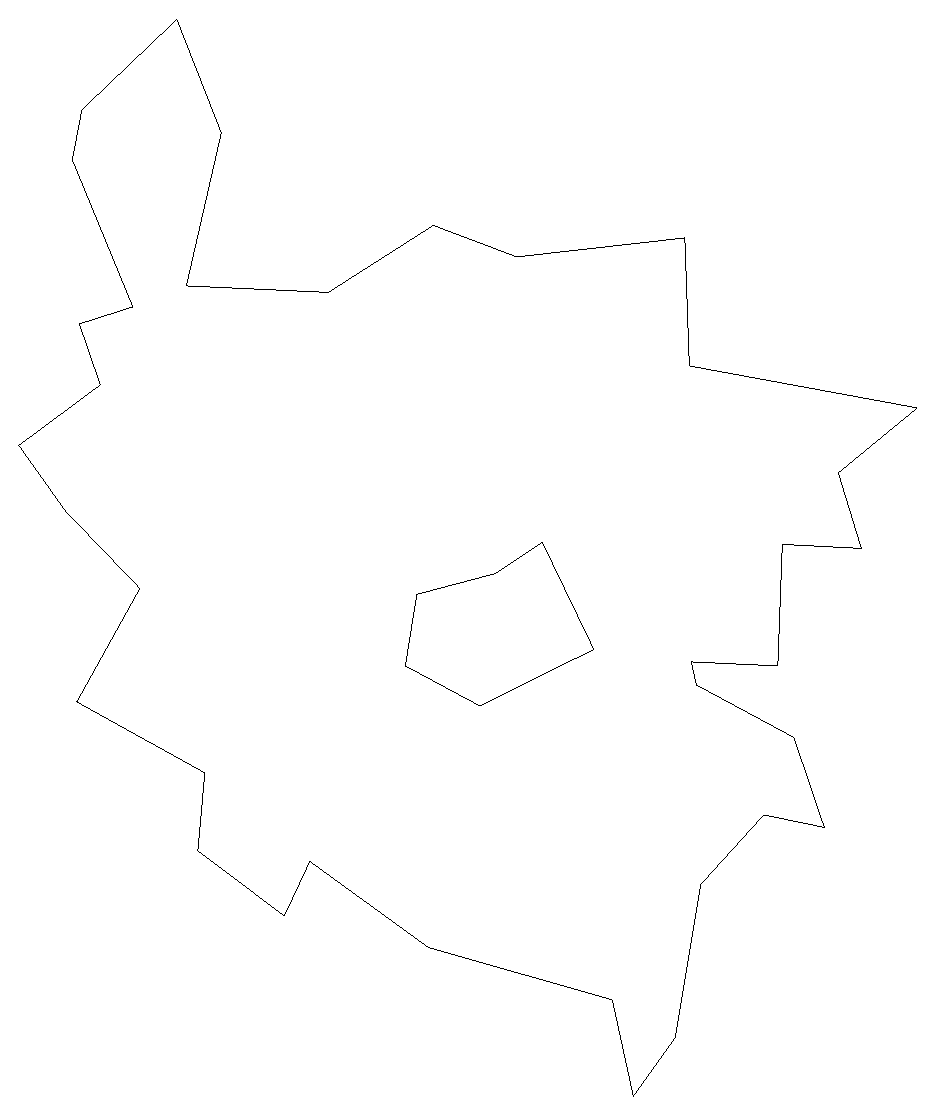
\includegraphics [scale=0.3]{grafiken/westin.eps}
{\em\caption{\label{westin} Example for a region that is totally
surrounded by another region}}
\end{figure}



Finally, we want to draw attention to an important limitation in
the current version of {\em BayesX}. In most cases {\em map
objects} serve as auxiliary objects to estimate spatial effects
with {\em bayesreg objects} or {\em remlreg objects}. In this case the names of the regions
of the map and the values of the spatial covariate, whose effect
is estimated, must match. Since there are only numerical variables
allowed in {\em dataset objects} (and no string valued variables),
the names of the regions in the corresponding {\em map object}
must necessarily be numbers, although there is in principle no
limitation for the names of regions in {\em map objects}.

\subsubsection*{Structure of a graph file}

A graph file stores the nodes and the edges of a graph $G =
(N,E)$, see for example George and Liu (1981, Ch. 3) for a first
introduction into graph theory. A graph is a convenient way of
representing the neighborhood structure of a geographical map. The
nodes of the graph correspond to the region codes. The
neighborhood structure is represented by the edges of the graph.
In some situations it may be useful to define weights associated
with the edges of a graph which can be stored in the {\em graph
file} as well.

We now describe the structure of a {\em graph file} as it is expected by
{\em BayesX}. The first line of a {\em graph file} must contain
the total number of nodes of the graph. In the remaining lines,
the nodes of the graph together with their edges and associated
weights are specified. One node corresponds to three consecutive
lines. The first of the three lines must contain the name of the
node, which may simply be the name of a geographical region. In
the second line the number of edges of that particular node is
given. The third line contains the corresponding edges of the
node, where an edge is given by the index of a neighboring node.
The index starts with zero. For example, if the fourth and the
seventh node/region in the {\em graph file} are
connected/neighbors, the edge index for the fourth node/region is
6 and for the seventh node/region 3.

We illustrate the structure of a {\em graph file} with an example. The
following few lines are the beginning
of the {\em graph file} corresponding to the map of (former) West Germany:

\footnotesize

327 \\
9162 \\
3 \\
1 2 3 \\
9174 \\
6 \\
0 4 2 3 5 6 \\
9179 \\
6 \\
0 1 7 3 8 6

\hspace{1cm} $\vdots$

\normalsize

\vspace{0.5cm}

The first line specifies the total number of nodes, in the present
example 327 nodes. The subsequent three lines correspond to the
node with name '9162', which is the first region in the map of
West Germany. Region '9162' has 3 neighbors, namely the second,
third and fourth node appearing in the graph file. Once again,
note that the index starts with zero, i.e. 0 corresponds to the
first node, 1 corresponds to the second node and so on. Lines 5 to
7 in the example correspond to node '9174' and its neighbors and
lines 8 to 10 correspond to node '9179'.

In a {\em graph file} it is also possible to specify weights associated
with the edges of the nodes. Since in the preceding example no
weights are explicitly specified, all weights are automatically
defined to be equal to one. Nonequal weights are specified in the
{\em graph file} by simply adding them following the edges of a
particular node.
An example of the beginning of a {\em graph file} with weights is given below:

\footnotesize

327 \\
9162 \\
3 \\
1 2 3 0.4 1.2 0.7\\
9174 \\
6 \\
0 4 2 3 5 6 0.4 0.3 0.8 0.8 1.4 1.6\\
9179 \\
6 \\
0 1 7 3 8 6 1.2 0.8 0.2 1.8 1.7 1.3

\hspace{1cm} $\vdots$

\normalsize

\vspace{0.5cm}

Here the edges of the first node '9162' have weights 0.4, 1.2 and
0.7.

\subsection*{Options}

\begin{itemize}
\item {\bf graph} \\
If #graph# is specified as an additional option, {\em BayesX}
expects a {\em graph file} to be read in rather than a {\em
boundary file}.
\item {\bf weightdef=adjacency $|$ centroid  $|$ combnd } \\
\label{weightsmap} Option #weightdef# allows to specify how the
weights associated with each pair of neighbors are computed.
Currently there are three weight specifications available,
#weightdef=adjacency#, #weightdef=centroid# and
#weightdef=combnd#. If #weightdef=adjacency# is specified, for
each pair of neighbors the weights are set equal to one. The so
called adjacency weights are the most common ones in spatial
statistics. Specifying #weightdef=centroid# results in weights
proportional to the distance of the centroids of neighboring
regions. More specifically, the weight $w_{us}$ of two neighboring
regions $u$ and $s$ is set to $w_{us} = c \cdot \exp(-d(u,s))$,
where $d$ is the Euclidian distance between the centroids of the
two sites and $c$ is a normalizing constant. The constant $c$ is
chosen in such a way that the total sum of weights is equal to the
total number of neighbors, which is in analogy to adjacency
weights. The third choice #weightdef=combnd# results in weights
proportional to the length of the common boundary. Similarly to
#weightdef=centroid#, the weights are normalized, i.e. the total
sum of weights is equal to the number of neighbors.

Note that the specification of the #weightdef# option is only
meaningful if a {\em boundary file} is read. If a {\em graph file}
is read  instead, the option has no effect because the boundary
information of regions is missing and  the computation of weights
is therefore impossible.
\end{itemize}



\section{Method outfile}
\label{mapoutfile} \index{map object!outfile command}

\subsection*{Description}

Method #outfile# performs the reverse of the #infile# command.
Using method #outfile#, the map information currently in memory is
written to an external file. The map information can be written
either in {\em boundary file} or in {\em graph file} format.

\subsection*{Syntax}

#> # {\em objectname}.#outfile# [{\em , options}] #using# {\em filename}

#outfile# writes the map information to the external file
specified in {\em filename}. The file format can be either a {\em
boundary file} or a {\em graph file}. If #graph# is specified as
an additional option, the file format will be a {\em graph file},
otherwise a {\em boundary file}.

\subsection*{Options}

\begin{itemize}
\item {\bf graph} \\
Forces the program to store the map information in {\em graph
file} format rather than {\em boundary file} format.
\item {\bf includeweights} \\
Option #includeweights# is meaningful only if the storing format
is a {\em graph file}, i.e. option #graph# is additionally
specified. In that case the weights associated with the edges
(neighbors) of the nodes (regions) are additionally stored.
\item {\bf replace} \\
The #replace# option allows {\em BayesX} to overwrite an already
existing file. If #replace# is omitted in the optionlist and the
file specified in {\em filename} already exists, an error will be
raised. This prevents you from overwriting an existing file
unintentionally.
\end{itemize}


\section{Method reorder}
\label{mapreorder} \index{reorder regions of a map} \index{map
object!reorder command}

\subsection*{Description}

Method #reorder# reorders the regions of a map in the sense that
the adjacency matrix of the reordered map has the smallest
envelope when compared to all other possible orderings. A new map
should always be reordered before using it with {\em bayesreg
objects} because MCMC block moves for spatial covariates will be
much faster if the envelope of the posterior precision matrix is
small, see \autoref{bayesregress}. For reordering of the regions
of the map the reverse Cuthill Mc-Kee algorithm is used, see
George and Liu (1981) p. 58 ff.

\subsection*{Syntax}

#># {\em objectname}.#reorder#

#reorder# reorders the regions of a map in order to obtain
smallest envelope of the corresponding adjacency matrix.

\subsection*{Options}

Not allowed.

\subsection*{Reference}

\begin{description}

\item[George, A., Liu, J. W. (1981).] {\em Computer Solution of Large
Sparse Positive Definite Systems.} Series in computational
mathematics, Prentice--Hall.

\end{description}
